\section{Approach}
Our approach was to use a Long Short Term Memory neural network. 
Long Short Term Memory networks are a special kind of RNN, capable of learning long-term dependencies~\cite{Hochreiter1997}. 
They work tremendously well on a large variety of problems (such as sentiment analysis) and are now widely used. Their architecture allows for the accumulation of information during operation and uses feedback to remember previous network call states~\cite{Christopher2015}.

Figure~\ref{fig:approach_model} demonstrates the architecture of the neural network.

\begin{figure}[H]
    \centering
    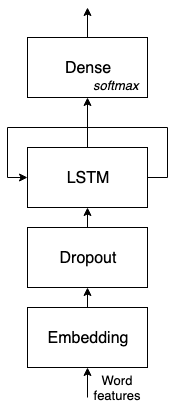
\includegraphics[width=0.25\textwidth]{approach_model}
    \caption{Long Short Term Memory for clickbait
    prediction}
    \label{fig:approach_model}
\end{figure}

Given an article whose title contains $N$ tokens, we first mapped each token $w_n$, where $n \in [1, N]$, to its corresponding word embedding $x_n$, through a word embedding matrix $W_E \in \mathbb{R}^{V \times d_0}$, where $d_0$ denotes the dimensionality of the word embedding, $V$ denotes the size of the vocabulary. 

After that, we used an uni-directional LSTM to encode the contextual information into its hidden state:
\[
    \vec{h_n} = LSTM(x_n, \vec{h_{n-1}}),
\]
where $\vec{h_n} \in \mathbb{R}^{d_1}$.

The token level attention vector $\alpha \in \mathbb{R}^N$, which represents the weights of tokens the title when predicting the annotation distribution, can be calculated as:
\[
    \alpha = softmax(\tanh(H W_H) \cdot v),
\]
where $H = \{ h_1, h_2, \dots, h_N \}$ and $H \in \mathbb{R}^{N \times 2d_1}$.

The vector representation of the tweet’s title can be calculated as:
\[
    s = H^T \alpha,
\]
where $s \in \mathbb{R}^{2d_1}$.

The predicted annotation distribution of this tweet on two categories $p = { p_1, p_2 }$ can be calculated as:
\[
    p = softmax(W_s s + b_s),
\]
where $W_s \in \mathbb{R}^{4\times 2d_1}$ and the bias term $b_s \in \mathbb{R}$ are the parameters to train.
